\documentclass[10pt]{article}
\usepackage{graphicx}
%\usepackage{fullpage}
\usepackage{setspace}
%%%%%\usepackage{lineno}
\usepackage[margin=3.2cm]{geometry}

\begin{document}
\begin{spacing}{1.5}

Hello everyone,

Diane's idea of fitting rainfall to a statistical distribution, and
manipulating the parameters of that distribution, really caught my
imagination.  I started to sketch out how I picture it working, and
ended up with the following simulation in R.  I thought the results
might be interesting, so I'll describe what I did.

First, I imagined that, since Diane had simulated 92 values, that she
had intended them to be evenly spaced at 4 day intervals over an
entire year.  I see from the mailing list that in fact we are
considering a 60 day experiment, but I think that, for the sake of
just exploring the idea in a simulation, the duration isn't too
important.

In my simulations, I used the same range of parameters that Diane
suggested in her email.  I simulated 92 values from the negative
binomial distribution and assigned each to a ''water day'' (at 4 day
intervals) in a random sequence.  I also imagined that the bromeliads
dry out every day, losing 2 percent of their volume daily (this is
probably too high?).  The bromeliads are visited every fourth day by a
perfectly responsible graduate student, who measures the quantity of
water and adds the amount prescribed by the distribution (which may
be 0).  On unwatered days the bromeliads continue to dry.

\begin{figure}
  \centering
  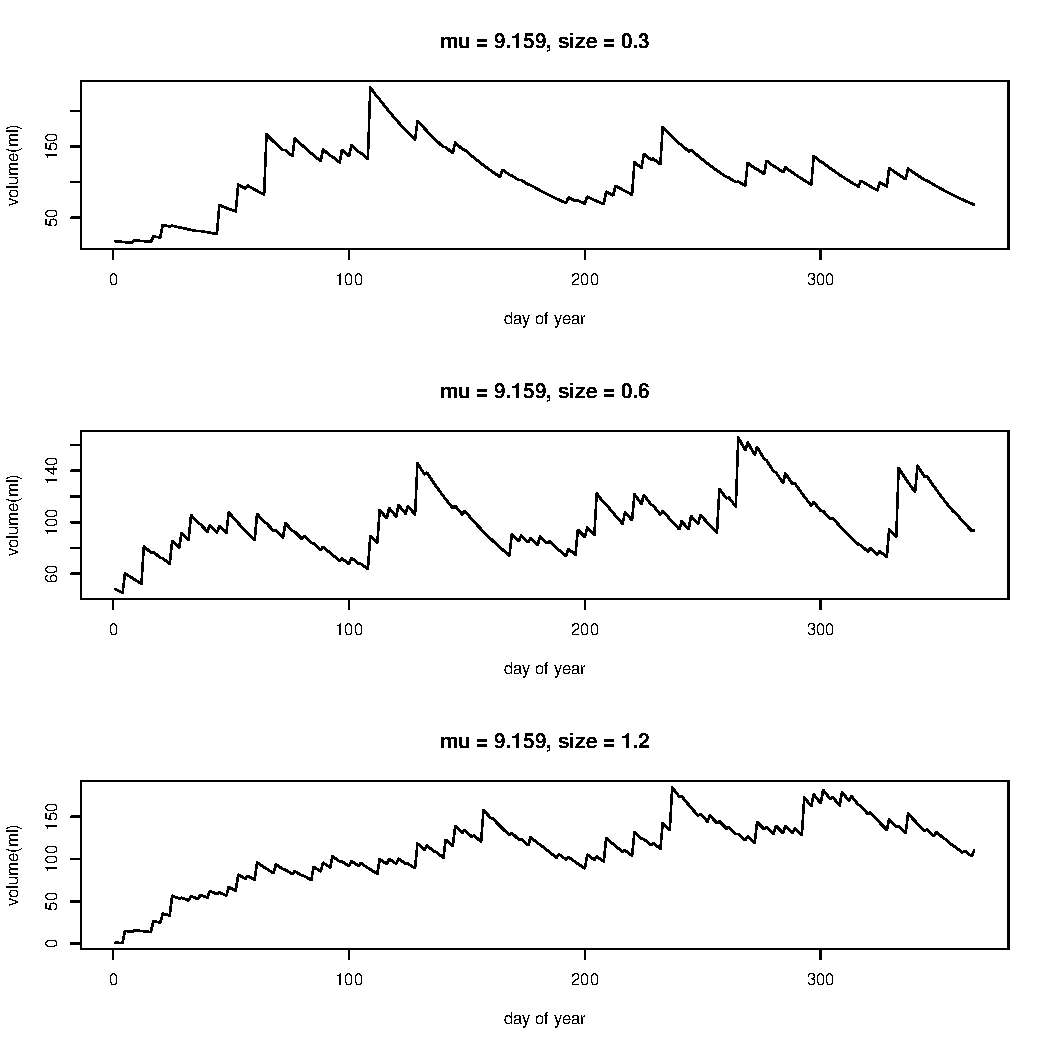
\includegraphics[width=0.6\textwidth]{singlebrom.pdf}
  \caption{Variation in water level within one year.  The parameter
    estimates represent the observed for Costa Rica, with various
    values of k.  (i.e. parameter values corresponding to the center
    column in the table that Diane sent)}
\end{figure}

The spiky lines here show how the water level in three bromeliads
might change in this kind of scenario. Its a really rudimentary
simulation: bromeliads start from empty, and have no maximum size.

I think we were discussing collecting some aggregate data on water
levels, such as average water content.  In these simulations, our
dutiful grad student measures the water just before adding more.
So, our data on mean water content represents the low point before
each spike.  


\begin{figure}
  \centering
  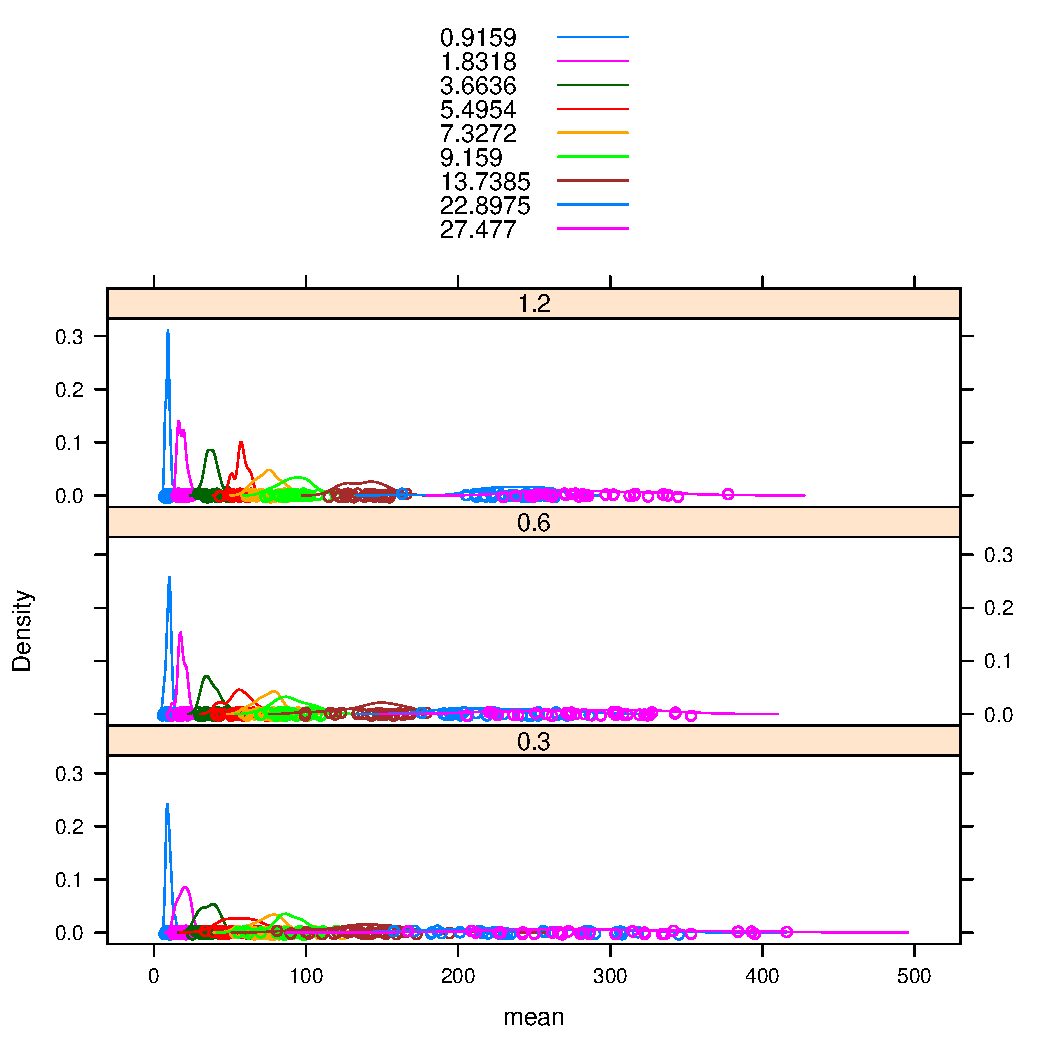
\includegraphics[width=0.6\textwidth]{meanannual.pdf}
  \caption{Mean annual variation in water content for 30 bromeliads in
    each combination of parameter values.  Within each panel, the
    different colours represent different values of mu (see key).  the
    different panels are different values of k.}
\end{figure}


We can calculate the mean water content of a bromeliad under all the
pairs of parameters that Diane suggested (Figure 2).  Each density
curve represents 30 bromeliads.  It seems like, even with very large
sample sizes, there can be large variation within treatments when mu is
large.

I was also interested by Regis and Ignacio's comments about the
\emph{sequence} of water additions.  Again focusing on mean water
content, I made a graph of mean water volume as a function of total
water volume (Fig 3)

\begin{figure}
  \centering
  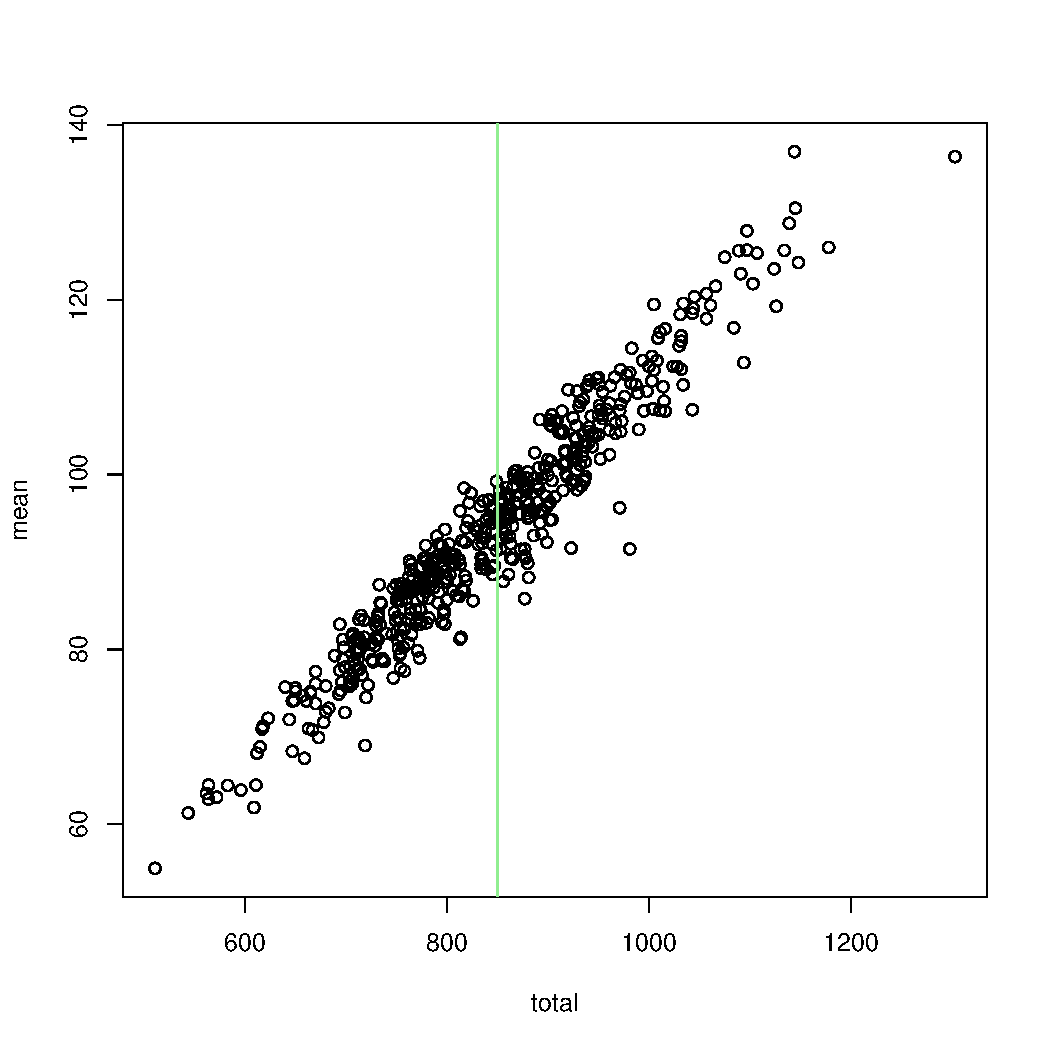
\includegraphics[width=0.6\textwidth]{totalmean.pdf}
  \caption{500 simulations of the relationship between the total
    amount of rain that falls in a year, and the average water content
    of the bromeliad.  Because each simulation is drawn at random,
    they vary in their total water content (x axis).  Within a given
    total rainfall amount (e.g. green line), variation in mean
    bromeliad capacity is entirely due to how much time the bromeliad
    spends drying out -- which may vary, depending on how many
    low-precipitation days happened to occur consecutively. parameters
    are constant for all simulations: mu = 9.159, k=0.6}
\end{figure}

I completely agree that there may be important biological consequences
to the timing of rainfall (e.g. how much water is present during the
breeding window of a certain population).  However, I thought it was
interesting to see that there can be quite a lot of variation in
something as basic as mean annual water content, just based on how
much time the bromeliad spent drying out.  

Perhaps we are actually trying to vary too much.  Varying the number
of rainy days, as well as the amount of rainy days, is already quite a
lot.  Maybe we should try to hold the sequence in which they occur
relatively constant.  Here's one possibility:
\begin{itemize}
\item first simulate all the rain amounts: all the replicates, in all
  the parameter combinations we intend to use
\item within each of these simulated ''yearly rainfalls'', score each
  rainy day with a percentile
\item calculate the mean amount of rain on each calendar day for the
  last ten years, and transform these into percentiles too
\item map the simulated rain onto calendar dates, using the observed
  percentiles as a guide.
\end{itemize}

What I'm trying to imagine is a way to put the rainiest days and the
driest days in the same order within all treatments.  So, on the
''rainiest day'', one bromeliad might get 70ml, while another only
gets 30ml -- but both cases it is the maximum rain they will get in
the entire experiment, and they get it on the same day.  Mapping this
sequence onto natural rainfall might not be necessary (for many sites,
the natural variation probably looks pretty random!) -- but having
some standard among all replicates and treatments seems like a good
idea.

I haven't done much playing with drying rate to see what effect that
has on any of these patterns.  I thought I would see what everyone
thinks before getting too carried away.  Thoughts?


\end{spacing}

\end{document}
